%************************************************
\chapter{Texture Features}\label{ch:texture}
%************************************************
\section{Introduction}
Texture is a household word outside image processing or related fields. However, in that context, it lacks a definition that allow us to measure and quantify it. Patter recognition provides us with a mathematical definition that allow us to use texture as a feature in our \ac{CAD} systems. 

Texture analysis is defined as any procedure by which we can quantify and classify the spatial variation of intensity throughout an image. In neuroimaging, texture has been widely used in segmentation (tissue classification) of \ac{MRI} images \cite{Saeed2002,Alejo2003,Wang2009}, although there exist a number of works using it for feature extraction in \ac{CAD}-like systems, like the works in \cite{kovalev2001three,sikio2015mr}, or our work on \ac{PKS} feature extraction \cite{Martinez-Murcia2013266,martinez2014parametrization}. 

Texture features can be classified in first, second and higher order analysis, depending on the number of variables used. First order statistics \cite{Martinez-Murcia2016b} are the most basic form of texture analysis, computing values such as average, variance or histogram of voxel intensity values \cite{Srinivasan2008}. 

The most popular form, with a very developed theoretical background, is second-order statistical texture analysis. This particular form is based on the probability of finding a pair of similar intensities at a certain distance and orientation of a certain image. From these probabilities, many measures can be derived, being the most popular the Haralick texture analysis \cite{Haralick73}. 

\begin{figure}[htp]
\centering
\includegraphics[width=0.9\linewidth]{Graphics/ch5/01-flowdiagram}
\caption[Schema of the proposed Texture-based CAD system.]{Schema of the proposed Texture-based \ac{CAD} system, including an optional feature selection block.}
\label{fig:textureCAD}
\end{figure}

In this work we have used Haralick texture analysis to extract features from DaTSCAN images and perform an automatic diagnosis of \ac{PD}. It follows the pipeline depicted at Figure~\ref{fig:textureCAD}, as in \cite{Martinez-Murcia2013266,martinez2014parametrization}. First we will provide an introduction to the methodology followed at Section~\ref{sec:methodsCh5}, including the volume selection tools, the Haralick texture analysis and the experiments used to validate the system. Later, in Section~\ref{sec:ch5results} we define the experiments and show their results. Finally, at Section~\ref{sec:ch5discuss} we discuss the implications of this systems and the evaluation results of our texture-based \ac{CAD} system.

\section{Methodology}\label{sec:methodsCh5}

\subsection{Volume selection}\label{sec:volume}
Even the registered DaTSCAN images contain many voxels that are outside the brain. Therefore, to obtain a more robust estimation of the texture, it would be desirable to perform the computation of the features on subvolumes of those images (or subimages) that contain only voxels inside the brain. Many strategies can be performed for this, for example, force the computation of the \ac{GLCM} to ignore background voxels. 

In this work, we opted for extracting a subvolume which contains only voxels higher than a certain intensity threshold $I_{th}$, which should be specified. To do so, we obtain the maximum and minimum coordinates for which $\mathbf{I}$ is higher than the threshold: 
\begin{align}
	p_{x,min} & = \argmin_x \left( \mathbf{I} > I_{th} \right)\\
	p_{x,max} & = \argmax_x \left( \mathbf{I} > I_{th} \right)
\end{align}

And we do the same for the $y$ and $z$ axis of the array. Once this is computed, we can select the volume by: 

\begin{equation}
	\mathbf{I}_{sub} = \mathbf{I}[p_{x,min}:p_{x,max}, p_{y,min}:p_{y,max}, p_{z,min}:p_{z,max}]
\end{equation}

The resulting subvolume $\mathbf{I}_{sub}$ is the minimum box-shaped volume containing all the values for which $\mathbf{I}>I_{th}$, which allow us to select a $I_{th}$ so that only the regions of interest are contained within. 

Different subimages and sizes are obtained when applying different $I_{th}$ In Figure~\ref{fig:comparisonIth} we depict a comparison between the resulting images for $I_{th} = [0.25, 0.30, 0.35]$. 

\begin{figure}
	\centering
	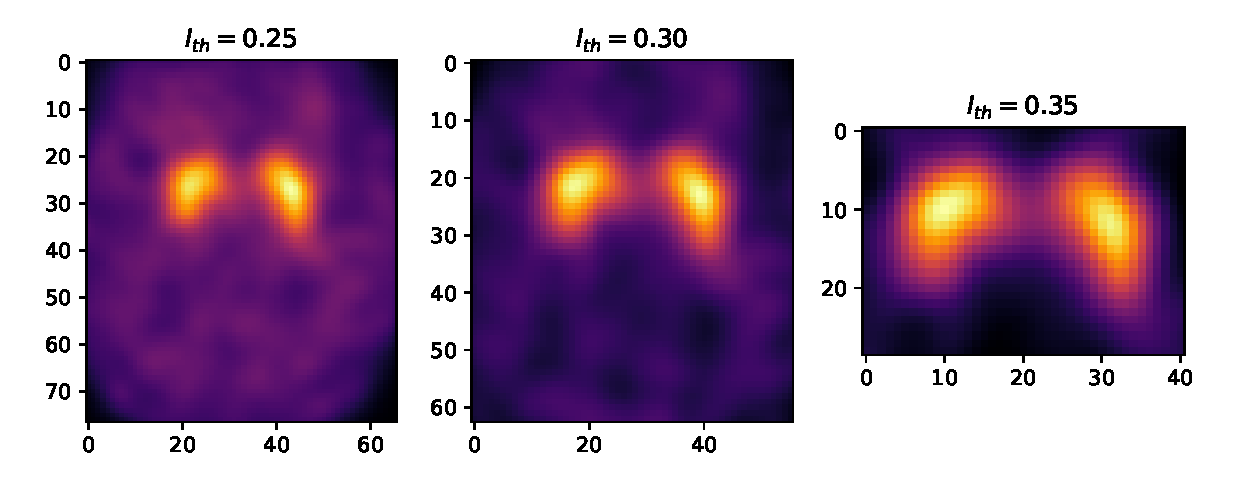
\includegraphics[width=0.90\columnwidth]{Graphics/ch5/comparisonIth.eps}
	\caption[Comparison of the different $I_{th}$ values.]{Comparison of the different $I_{th}$ values for a random subject extracted from the PPMI database.}
	\label{fig:comparisonIth}
\end{figure}

\subsection{Haralick Texture Analysis}\label{sec:haralick}
\subsubsection{Gray Level Co-occurrence Matrix}
%Que son las matriz de coocurrencia y las texture features
The Haralick texture analysis is based on the computation of a \acf{GLCM}, which is a form of evaluating second-order texture statistics. This matrix is a summary of the probabilities of finding a pair of similar grey levels at a certain distance and in a certain direction. 

The combination of the unitary vector dimension and the distance defines the offset $\Delta=(d_x,d_y,d_z)$, whose norm is the distance $d$ and is defined in a given spatial direction. In this work, we use a three-dimensional approach to the computation of the \ac{GLCM}, based on \cite{Philips2008}, that uses thirteen spatial directions to generalize the standard 2D \ac{GLCM} to 3D. These offset define different angles and are used to get some degree of rotational invariance \cite{Philips2008}. 

Medical images have different number precision, which can vary from regular 8bit integers (256 values) to the type float64 ($1.844\times10^{19}$ possible values). Using all these values, even in the smallest case, would lead to $256\times 256$ matrices, which would be both non representative of the real texture and computationally expensive. Therefore, prior to the \ac{GLCM} computation, we posterize the image, that is, the image is quantified to use only 16 grey levels. This leads to more tractable \ac{GLCM} without losing their representativeness. 

Once images have been posterized, for two different grey levels $i$ and $j$, the value of the co-occurrence matrix $\mathbf{C}$ over a $n \times m \times k$ three-dimensional image $\mathbf{I}$ is defined as: 
\begin{equation}\label{eq:cooc3D}
\mathbf{C}_{\Delta}(i,j)=\sum_{\mathbf{p}=(1,1,1)}^{(n,m,k)}\begin{cases} 1, & \mbox{if }\mathbf{I}(\mathbf{p})=i\mbox{ and }\mathbf{I}(\mathbf{p}+\Delta)=j \\ 0, & \mbox{otherwise}\end{cases}
\end{equation}
where $\Delta$ is the three dimensional offset that we defined previously, and $\mathbf{p}$ is the position of a given voxel inside the image. 

We will compute one $16\times16$ \ac{GLCM} for each of the combinations of direction and distances. This matrix $\mathbf{C}_{\Delta}$ is later modified to create the probability matrix $\mathbf{P}$ as: 
\begin{equation}
\mathbf{P}(i,j) = \frac{\mathbf{C}_{\Delta}(i,j)}{\sum_{i,j}\mathbf{C}_{\Delta}(i,j)}
\end{equation}
from which the texture features will be derived.

\subsubsection{Haralick Texture Features}\label{sec:haralickFeatures}
%Parámetros de haralick. 
In \cite{Haralick73,Haralick1992a}, many texture features are derived from the probability matrix defined above. We have selected twelve of these features to use in this work. These features are: 
\begin{align}\label{eq:energy}
\text{Energy} & = \sum\limits_i\sum\limits_j \mathbf{P}(i,j)^2\\ \label{eq:entropy}
\text{Entropy} & = \sum\limits_i\sum\limits_j \mathbf{P}(i,j) \log \mathbf{P}(i,j)\\\label{eq:correlation}
\text{Correlation} & = \frac{\sum_i\sum_j ij\mathbf{P}(i,j) - \mu_x\mu_y}{\sigma_x\sigma_y}\\\label{eq:contrastHar}
\text{Contrast} & = \sum\limits_{n=0}^{N_g-1} n^2 \left\lbrace\sum\limits_{|i-j|=n}\mathbf{P}(i,j)\right\rbrace  \\
\text{Variance} & \sum\limits_i\sum\limits_j (i-\mu_i)^2 \mathbf{P}(i,j)+ (j-\mu_j)^2\mathbf{P}(i,j)\\
\text{Sum Mean} & = \frac{1}{2} \sum\limits_i\sum\limits_j(i\mathbf{P}(i,j)+j\mathbf{P}(i,j))\\
\text{Inertia} & \sum\limits_i\sum\limits_j (i-j)^2\mathbf{P}(i,j)\\
\text{Cluster Shade} & \sum\limits_i\sum\limits_j (i+j-\mu_x-\mu_y)^3 \mathbf{P}(i,j)\\
\text{Cluster Tendency} & \sum\limits_i\sum\limits_j \{ i+j-\mu_x-\mu_y\}^4 \mathbf{P}(i,j)\\\label{eq:homogeneity}
\text{Homogeneity} & = \sum\limits_i\sum\limits_j \frac{\mathbf{P}(i,j)}{1+|i-j|}\\
\end{align}
\begin{align}
\text{Max Probability} & = \max_{i,j} \mathbf{P}(i,j)\\
\text{Inverse Variance} & = \sum\limits_i\sum\limits_j {\mathbf{P}(i,j) \over (i-j)^2}
\end{align}
where $\mu_i$, $\mu_j$, $\sigma_i$ and $\sigma_j$ are the column and row-wise mean and variance respectively. These feature measure things such as the randomness of the grey-level distribution (entropy), the number of repeated pairs (energy), the local contrast or homogeneity of the image, variance, the tendency to form clusters (cluster shade and tendency), among others. 

For this work we have used a distance $d$ ranging from 1 to 10, at each of the $13$ spatial directions. Therefore, we have computed $13\times10=130$ \acp{GLCM} per image, from which $12$ texture features are computed. Our final feature vector will therefore have $1560$ features in total. 

To further reduce the dimensionality of the feature vector, we have performed feature selection using the $t$-test, \ac{MWW} $U$-test and the relative entropy (\ac{KL} divergence) criteria (see Section~\ref{sec:featureSelection}). 

\subsection{Experiments}
For evaluating the system proposed in this chapter, combining texture analysis and other feature selection algorithms, we propose two experiments: 
\begin{itemize}
	\item Experiment 1: Ability of the different texture features to differenciate between \ac{PD} affected subjects and \acp{CTL}. Each of the texture features is analysed in two different ways: a ''single approach'', which only considers one type of feature using only the matrices at a distance $d$ from the central voxel -and using all the spatial directions- and a ''cumulative approach'' which considers one type of feature too, but this time using all matrices in distances ranging from 1 to $d$. 
	\item Experiment 2: Impact of the introduction of a feature selection algorithm (of those presented at Section~\ref{sec:featureSelection}) after computing the texture features. This allow us to pool all texture features at all distances and directions, and then select the most discriminative ones according to some of these criteria.  
\end{itemize}

All images used are intensity normalized using either normalization to the maximum or integral normalization (see Section~\ref{sec:intensityPrep}), and afterwards, a subvolume can be extracted using the intensity threshold methodology described at Section~\ref{sec:volume}. In addition to the feature extraction technique using texture analysis, and the feature selection procedure defined for Experiment 2, we use a linear \ac{SVC} for classifying, and 10-fold cross validation strategy (see Section~\ref{sec:validation} for more details). 

\section{Results}\label{sec:ch5results}
\subsection{Experiment 1}
In this experiment, the influence and effect of each texture feature is tested, as in \cite{Martinez-Murcia2013266}. We have tested the computation of the \acp{GLCM} over the image subvolumes using different thresholds $I_{th}$ (see Sec. \ref{sec:volume}) ranging from 0 to 50\% of the maximum intensity value, and a range of distances $d=1,2,\dots10$ in the thirteen spatial directions.

To check which value of the intensity threshold is the best for computing the texture features, we can compute the general tendency of the system by averaging the accuracy values. Figure~\ref{fig:featuresIth} depicts the general trend of the performance over the intensity threshold for either the no normalized or normalized images. This is done for the single and cumulative approach. 

\begin{figure*}% single and cumulative approach. 
	\centering
	\subfloat[No Normalization (Single)]{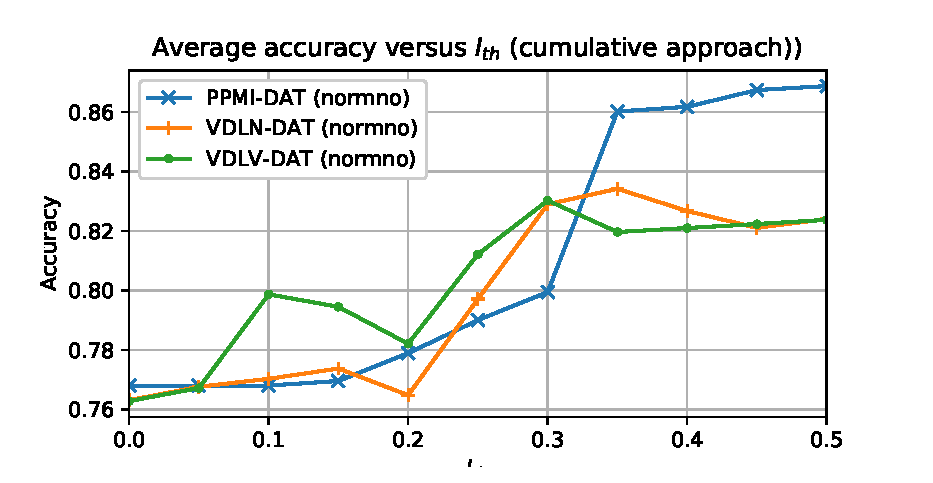
\includegraphics[width=0.5\textwidth]{Graphics/ch5/featuresIthdis_no.eps}\label{fig:acc_dist_no}}
	\subfloat[No Normalization (Cumulative)]{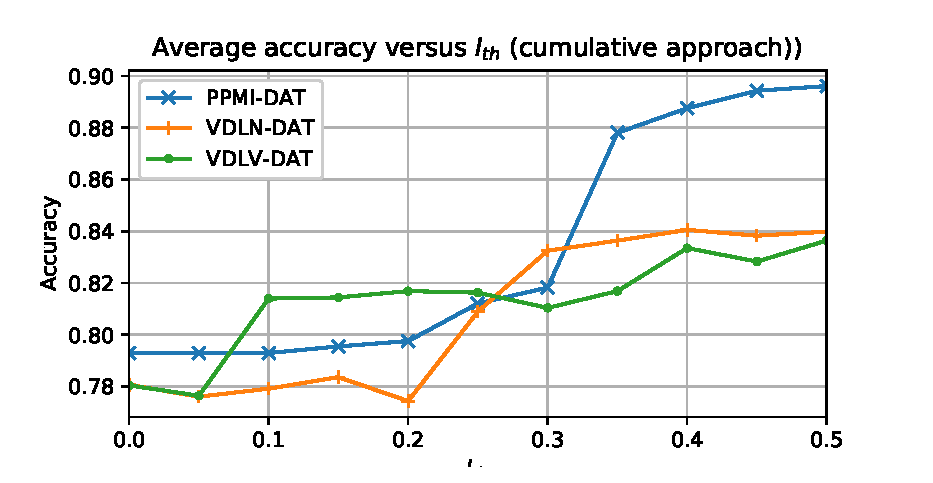
\includegraphics[width=0.5\textwidth]{Graphics/ch5/featuresIthcum_no.eps}\label{fig:acc_cum_no}}\\
	\subfloat[Maximum (Single)]{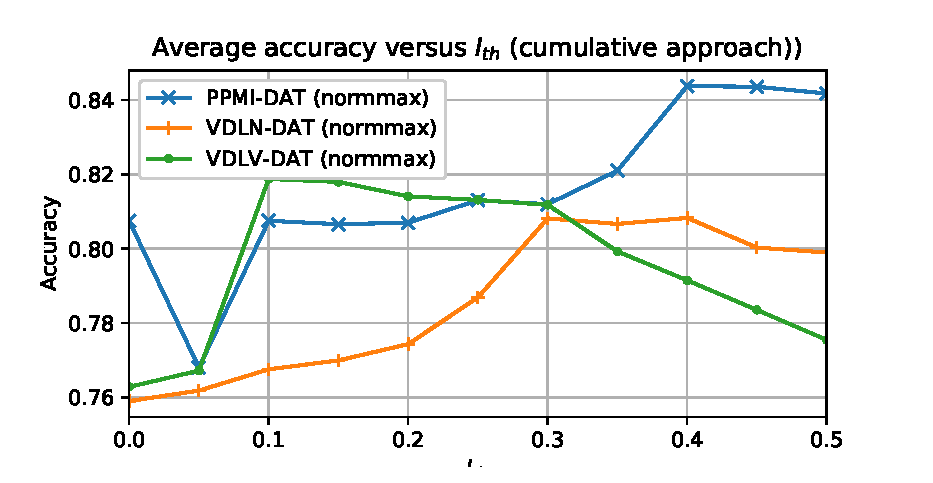
\includegraphics[width=0.5\textwidth]{Graphics/ch5/featuresIthdis_max.eps}\label{fig:acc_dist_max}}
	\subfloat[Maximum (Cumulative)]{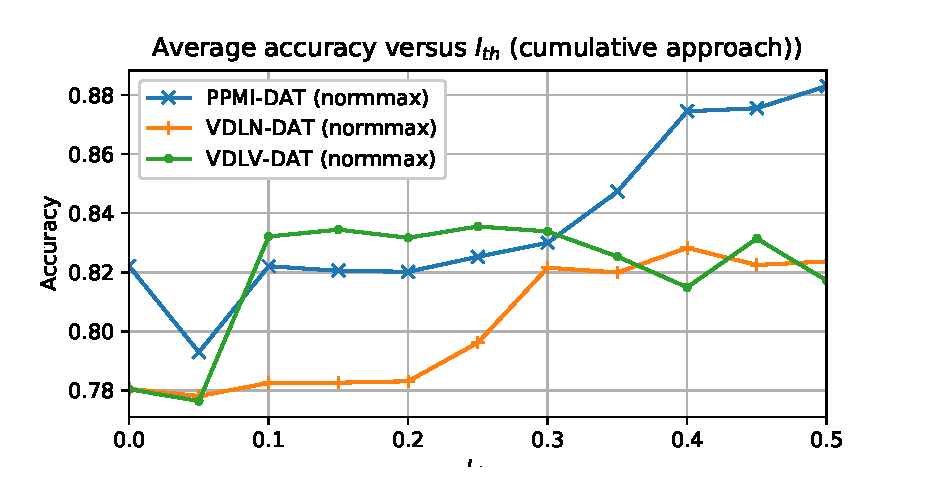
\includegraphics[width=0.5\textwidth]{Graphics/ch5/featuresIthcum_max.eps}\label{fig:acc_cum_max}}\\
	\subfloat[Integral (Single)]{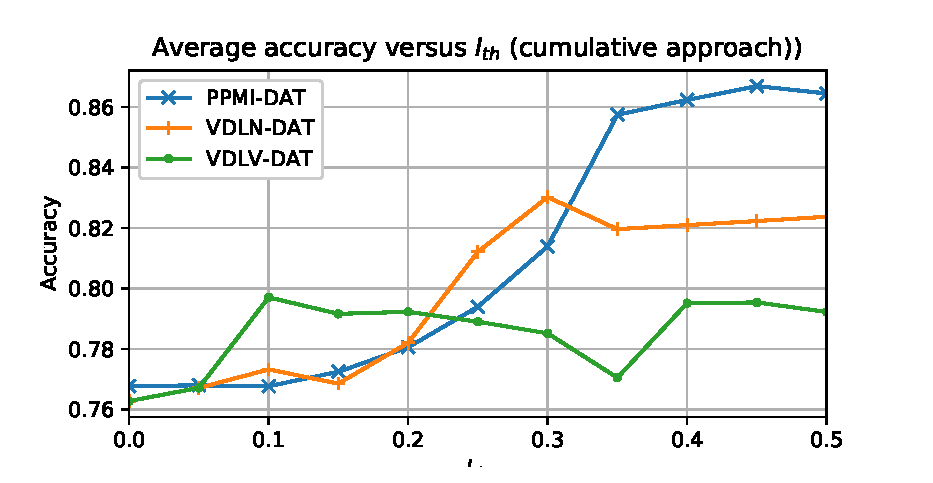
\includegraphics[width=0.5\textwidth]{Graphics/ch5/featuresIthdis_int.eps}\label{fig:acc_dist_int}}
	\subfloat[Integral (Cumulative)]{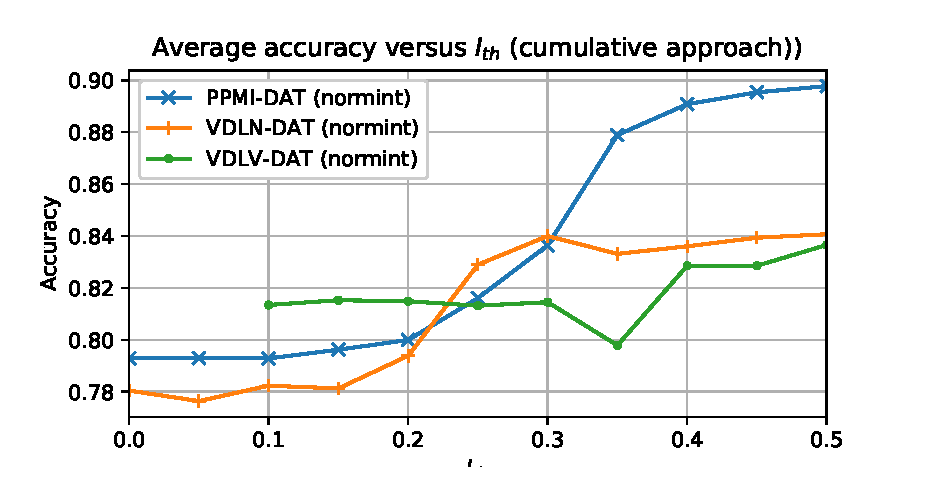
\includegraphics[width=0.5\textwidth]{Graphics/ch5/featuresIthcum_int.eps}\label{fig:acc_cum_int}}
	\caption[Evolution of the average accuracy with the intensity threshold.]{Evolution of the average accuracy values obtained for the single approach and the cumulative approach over the intensity threshold, using no normalization, normalization to the maximum and integral normalization.}
	\label{fig:featuresIth}
\end{figure*}

The most obvious differences can be found between normalization procedures. As a general trend, the integral normalization barely has an impact over the performance achieved with the registered images. Furthermore, the normalization to the maximum even drops the performance for high $I_{th}$, however it increases the general performance in the range 0.1-0.3. From these graphs it is patent that normalization has no impact on the performance achieved by our system, which can be consider an advantage, since it reduces the preprocessing needed. 

In this regard, the VDLV-DAT dataset has an strange behaviour. It performance holds and even increases when using normalization to the maximum, but significantly drops when integral normalization is used. This is exactly the opposite as happens to the other dataset, and will be discussed later.  

In these images, we can observe a strong dependence of the system's performance with the intensity threshold $I_{th}$. In general, the performance increases with a more restrictive threshold (a smaller box around the striatum). This increase is probably due to removing the background from the texture analysis. According to Figure~\ref{fig:comparisonIth}, a value between 0.30 a 0.35 could be indicative of a complete background removal from the computation. In most cases, $I_{th}\approx 0.35\times I_{max}$ seems to be a critical value: either the global maximum or the inflection point from which accuracy stabilizes. This would prove that eliminating the background is beneficial for the texture analysis and a posterior classification of the images. 

To obtain a deeper insight on the behaviour of each texture feature, we can use a violin plot. This plot is an evolution of the boxplot, frequently used in statistical distributions, in which the distribution of values is shown along with the mean and standard deviation of the set of given data. In our case, we show the violin plot of all accuracy values for each database, grouped by texture feature, at Figure~\ref{fig:features_acc}. Since the performance of the integral normalization was similar to applying no normalization at all, we have only used performance data for the databases normalized to the maximum and the original images. 

\begin{bigfigure}
	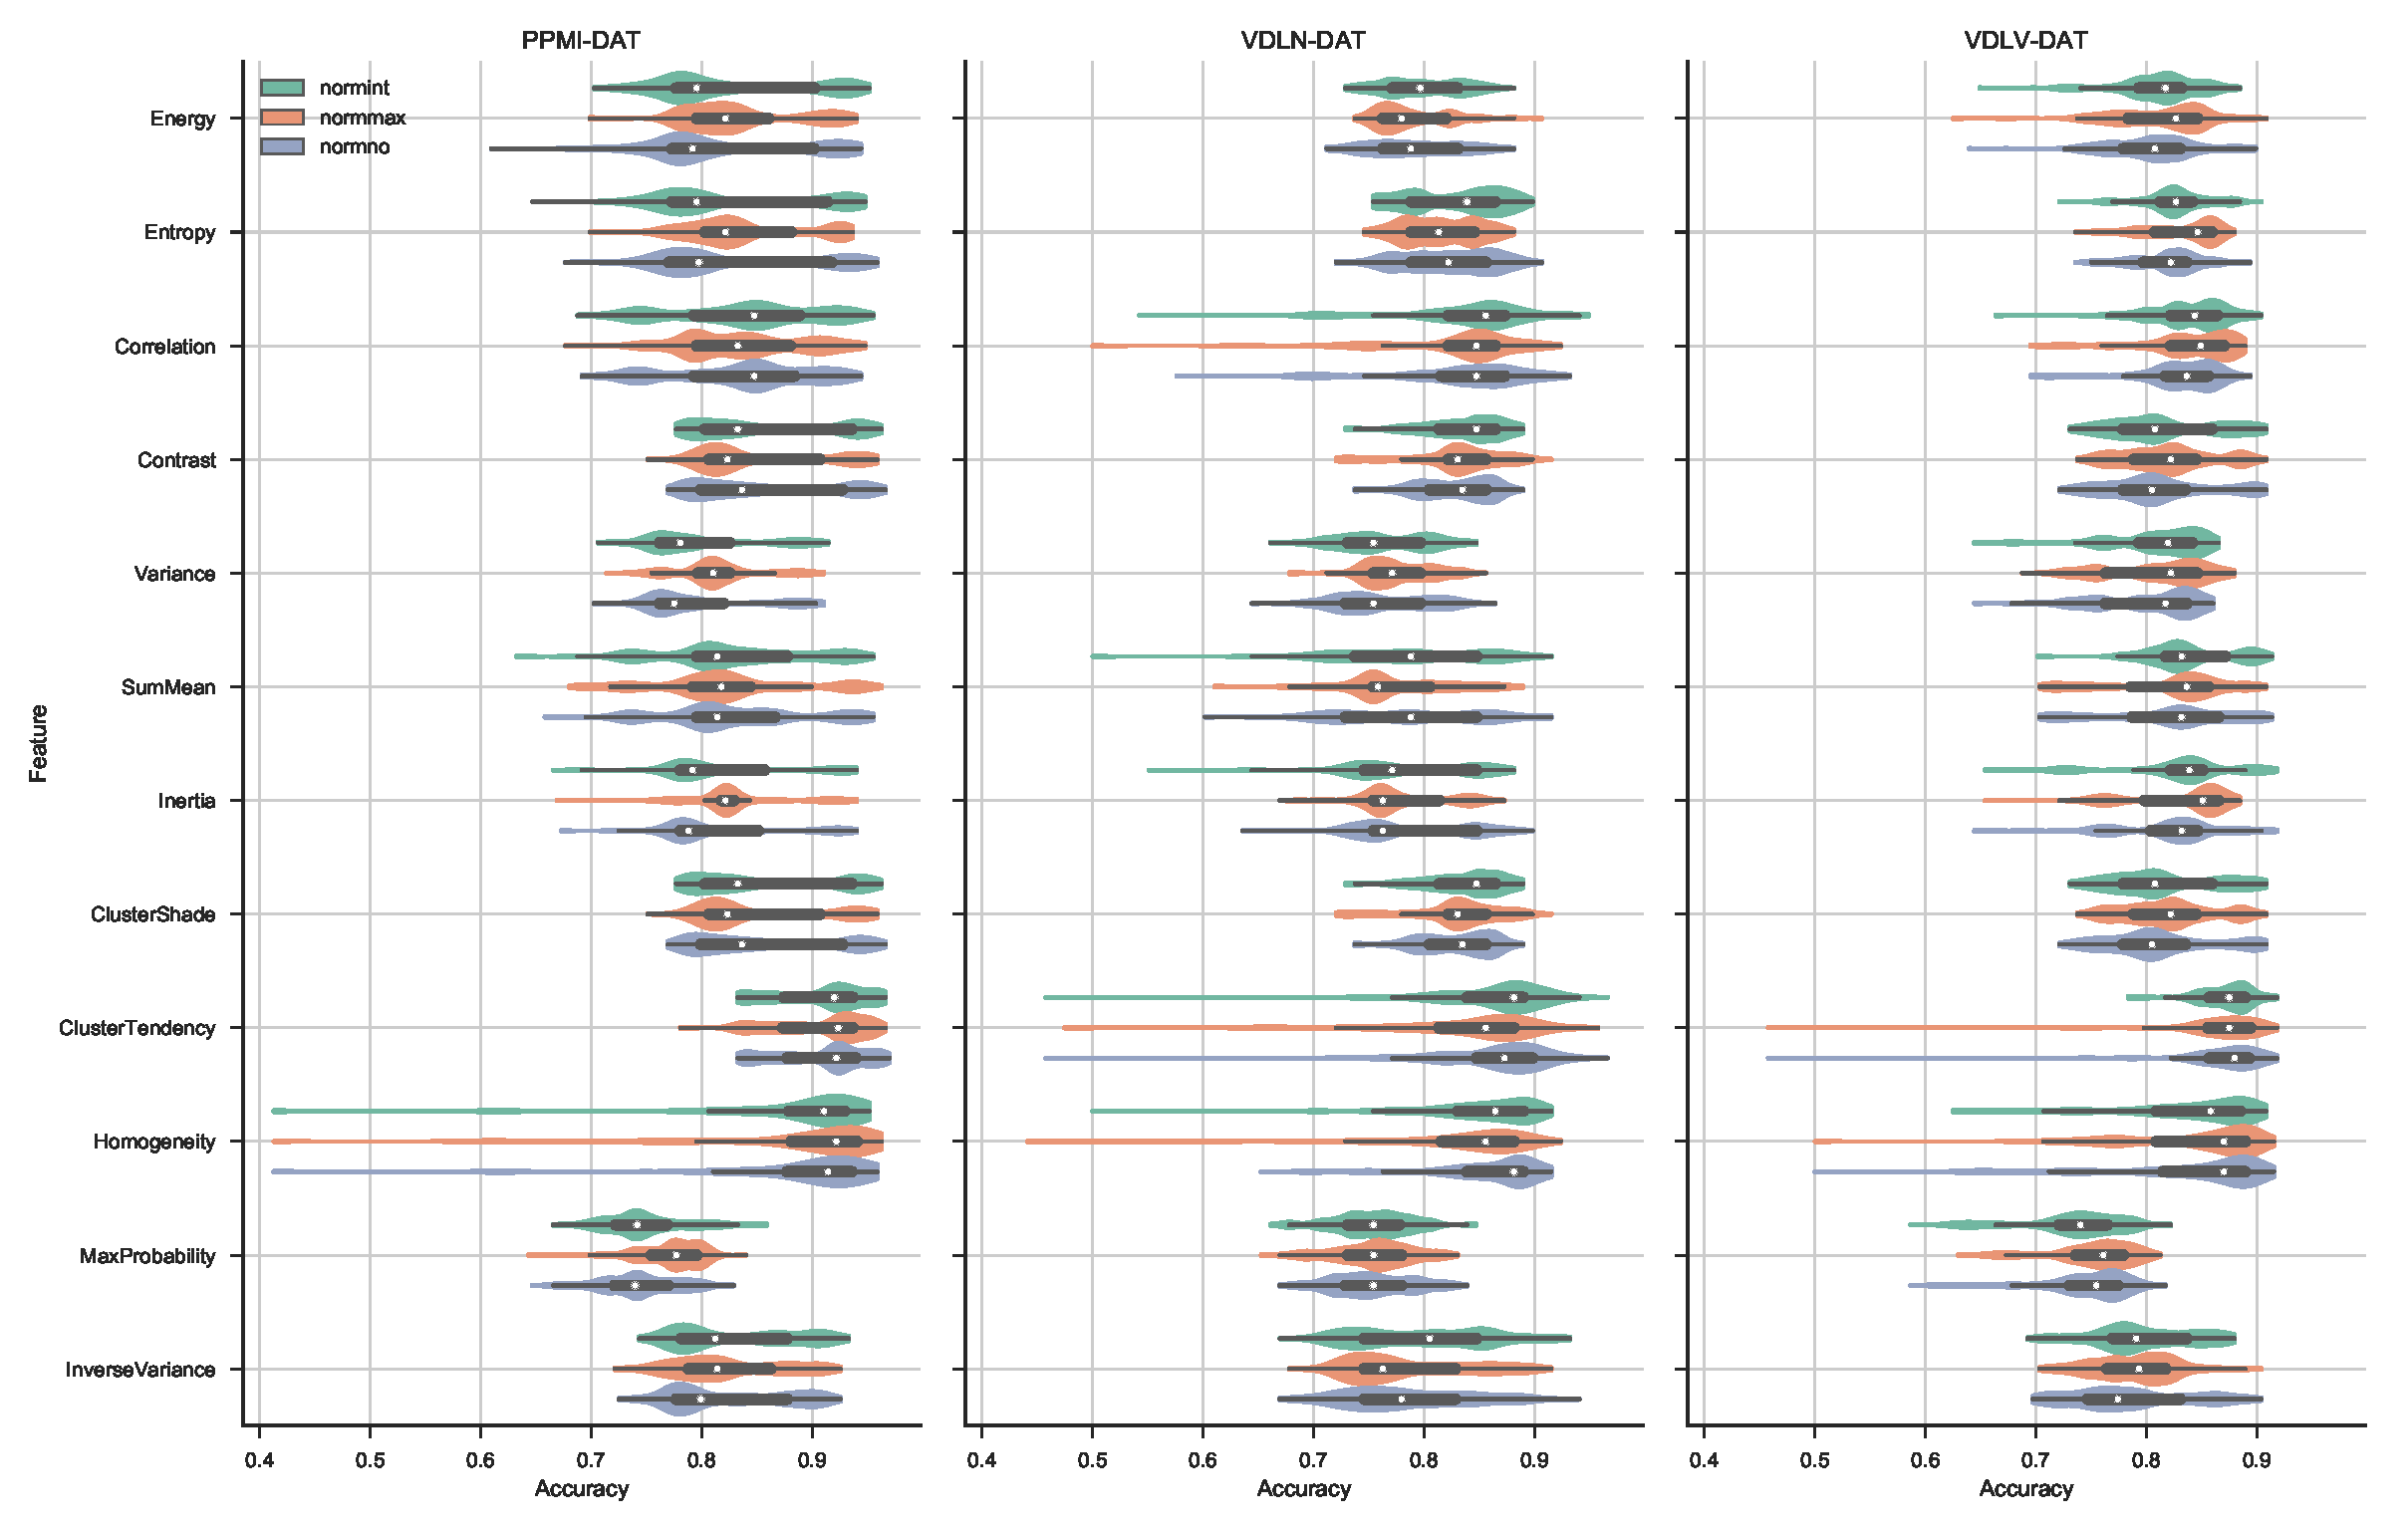
\includegraphics[width=\textheight]{Graphics/ch5/features_acc.eps}\label{fig:acc_distances}
	\caption[Violin plot of all accuracy values, grouped by database.]{Violin plot of all accuracy values, grouped by database and showing the differences between normalization to the maximum and the original images.}
	\label{fig:features_acc}
\end{bigfigure}

Figure~\ref{fig:features_acc} shows the differences between applying or not the normalization to the maximum (in colors), and also the differences in performance obtained depending on the database. We can observe that in average (the white dot), Cluster Tendency is the best performing feature. Homogeneity, Contrast and Correlation also achieve good results. This behaviour is consistent along all three databases, from which we can consider Cluster Tendency the most discriminant feature for \ac{PD} patterns. 

In Tables~\ref{tab:exp1AccSingle} and \ref{tab:exp1AccCumulative}, we take a look at the performance achieved by the maximum scoring feature in all databases with different normalization procedures. This is shown for both the single and the cumulative approach. 

\begin{table*}[htp]
	\centering
\begin{tabular}{llllllll}
	\toprule
	                          & Norm.    & Feature         & $I_{th}$ & $d$ & acc.  & sens. & spec  \\ \midrule
	\multirow{3}{*}{PPMI-DAT} & Original & Cluster Tendency & 45       & 8            & 0.952 & 0.946 & 0.956 \\
	                          & Integral & Cluster Tendency & 45       & 4            & 0.952 & 0.946 & 0.956 \\
	                          & Maximum  & Cluster Tendency & 45       & 8            & 0.948 & 0.955 & 0.943 \\\midrule
	\multirow{3}{*}{VDLN-DAT} & Original & Cluster Tendency & 40       & 1              & 0.941 & 0.956 & 0.932 \\
	                          & Integral & Cluster Tendency & 35       & 3            & 0.941 & 0.978 & 0.918 \\
	                          & Maximum  & Inverse Variance & 45       & 8            & 0.923 & 0.933 & 0.918 \\\midrule
	\multirow{3}{*}{VDLV-DAT} & Original & Cluster Tendency & 35       & 7            & 0.941 & 0.978 & 0.918 \\
	                          & Integral & Cluster Tendency & 30       & 6            & 0.904 & 0.889 & 0.920 \\
	                          & Maximum  & Cluster Tendency & 35       & 1              & 0.923 & 0.907 & 0.940 \\ 
	                          \bottomrule& 
\end{tabular}
	\caption[Maximum scoring feature (single approach).]{Maximum scoring feature for each combination of database and normalization procedure, and the intensity threshold and offset distance for which this maximum performance is achieved, using the single approach.}
	\label{tab:exp1AccSingle}
\end{table*}

\begin{table*}[htp]
	\centering
\begin{tabular}{llllllll}
	\toprule
	                          & Norm.    & Feature          & $I_{th}$ & $d$ & acc.  & sens. & spec  \\ \midrule
	\multirow{3}{*}{PPMI-DAT} & Original & Cluster Tendency & 45       & 6   & 0.970 & 0.982 & 0.962 \\
	                          & Integral & Cluster Tendency & 40       & 5   & 0.966 & 0.982 & 0.956 \\
	                          & Maximum  & Cluster Tendency & 45       & 5   & 0.966 & 0.982 & 0.956 \\ \midrule
	\multirow{3}{*}{VDLN-DAT} & Original & Cluster Tendency & 45       & 7   & 0.966 & 1.000 & 0.945 \\
	                          & Integral & Cluster Tendency & 45       & 7   & 0.966 & 1.000 & 0.945 \\
	                          & Maximum  & Cluster Tendency & 50       & 7   & 0.958 & 0.978 & 0.945 \\ \midrule
	\multirow{3}{*}{VDLV-DAT} & Original & Inertia          & 50       & 7   & 0.918 & 0.963 & 0.870 \\
	                          & Integral & Inertia          & 50       & 6   & 0.918 & 0.963 & 0.870 \\
	                          & Maximum  & Cluster Tendency & 45       & 7   & 0.918 & 0.944 & 0.890 \\ \bottomrule
	                          &
\end{tabular}
	\caption[Maximum scoring feature (cumulative approach).]{Maximum scoring feature for each combination of database and normalization procedure, and the intensity threshold and offset distance for which this maximum performance is achieved, using the cumulative approach.}
	\label{tab:exp1AccCumulative}
\end{table*}

The first noticeable feature is that, for both the single and cumulative approaches, the best scoring normalization method is using no normalization at all. As commented before, that will be discussed later. Secondly, as anticipated, the best scoring feature is Cluster Tendency in most cases, and the systems perform better when the intensity threshold is more restrictive. 

When comparing the single approach with the cumulative one, it is obvious that best results are obtained with the cumulative one, except for the particular case of the VDLV-DAT. Whereas with the single approach there was no evident choice for the offset distance $d$, in the cumulative one results are obtained combining the first 5-7 distances at which the \ac{GLCM} was computed. This is reasonable, since for the single approach we only use the features contained at each $d$, while in the cumulative approach we pool much more information for training and testing the system. Nevertheless, the single approach obtains decent results in many cases, which proves the value of the Haralick texture features for characterizing DaTSCAN images. 

\subsection{Experiment 2}
In experiment 2 we pool together all features derived from all \acp{GLCM}, and use a feature selection algorithm (see Section~\ref{sec:featureSelection}). This gives us 1560 features per subject, from a total 12 features computed at 13 directions and 10 distances. We will test how values such as $I_{th}$, the normalization algorithm or the percentage of selected voxels affects the performance of this system, and discuss the results. 

\begin{figure}[htp]
	\centering
	\subfloat[Original images]{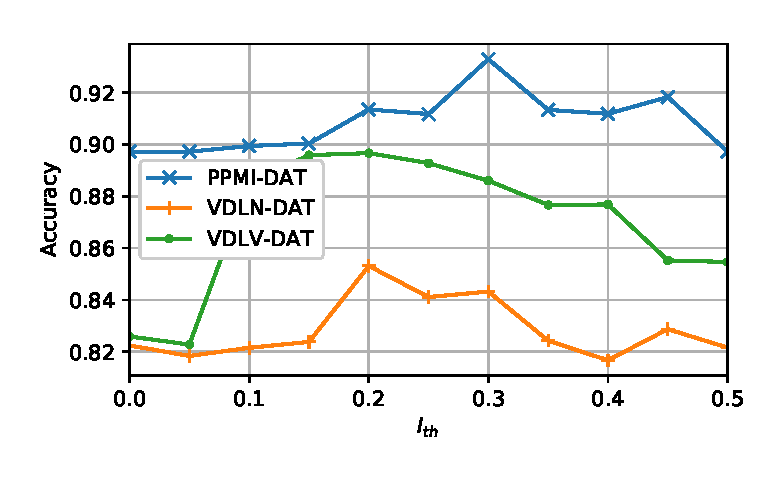
\includegraphics[width=0.5\textwidth]{Graphics/ch5/accuracyOverIth_no.eps}\label{fig:averageAcc_IthNorm_no}}
	\subfloat[Integral Normalization]{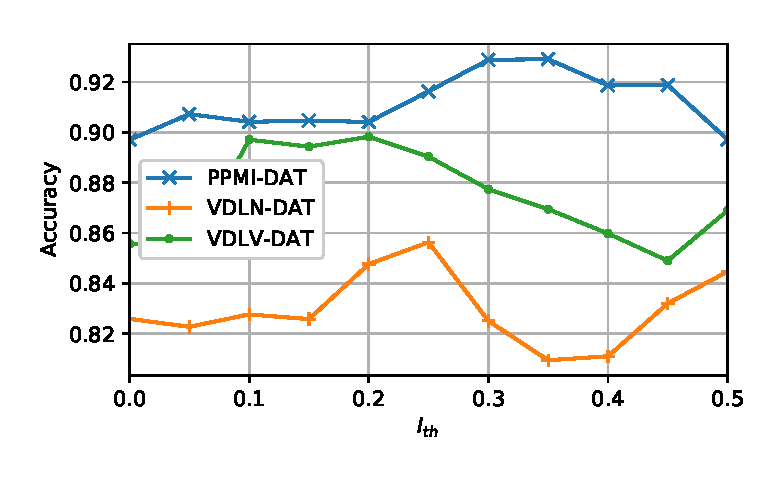
\includegraphics[width=0.5\textwidth]{Graphics/ch5/accuracyOverIth_int.eps}\label{fig:averageAcc_IthNorm_int}}\\
	\subfloat[Normalization to the Maximum]{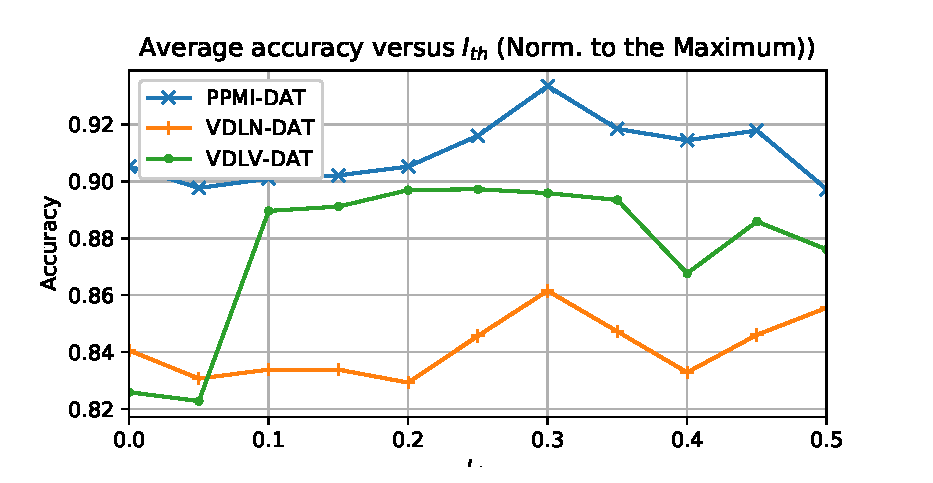
\includegraphics[width=0.5\textwidth]{Graphics/ch5/accuracyOverIth_max.eps}\label{fig:averageAcc_IthNorm_max}}
	\caption{Accuracy obtained by averaging all accuracy values using a given volume selection threshold $I_{th}$.}
	\label{fig:averageAcc_IthNorm}
\end{figure}

In Figure~\ref{fig:averageAcc_IthNorm} we show how the performance evolves when varying the $I_{th}$, as we did in Experiment 1, by displaying the average accuracy. As in the previous case, the integral normalization performs similarly to the original, non-normalized images. In this case, the normalization to the maximum strategy seems to affect more the VDLV-DAT dataset, slightly improving its performance. Again, best $I_{th}$ seems to be located at approximately 0.30 for all databases when using normalization to the maximum, although for other approaches, this happens with smaller $I_{th}$ (0.20 for VDLN-DAT and VDLV-DAT original images). For these values, there are still background voxels included in the computation of textures, but its negative influence might be overcome by the feature selection procedure. 

These results corroborate that our volume selection strategy is profitable in almost any case, using a intensity threshold between $0.25$ and $0.45$. 

\begin{figure*}
	\centering
	\subfloat[PPMI-DAT]{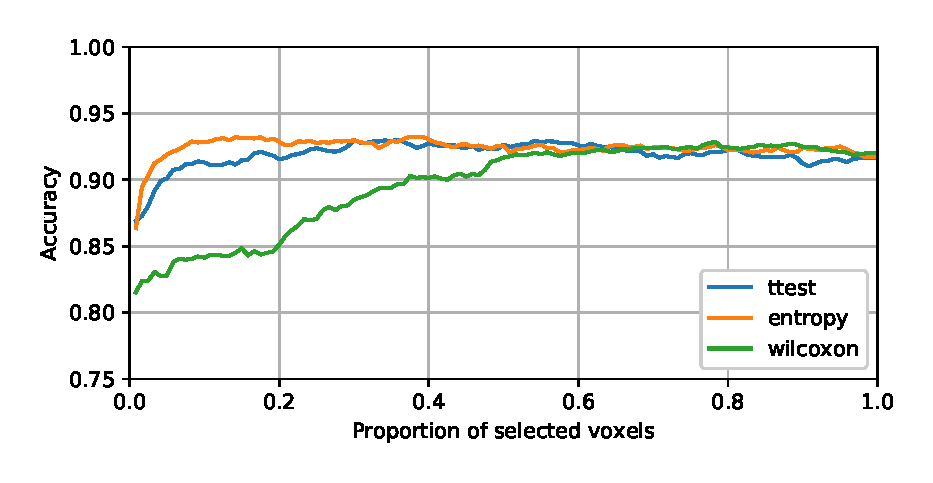
\includegraphics[width=0.5\textwidth]{Graphics/ch5/features_avAccPPMI.eps}\label{fig:experiment4-ppmi}}
	\subfloat[VDLN-DAT]{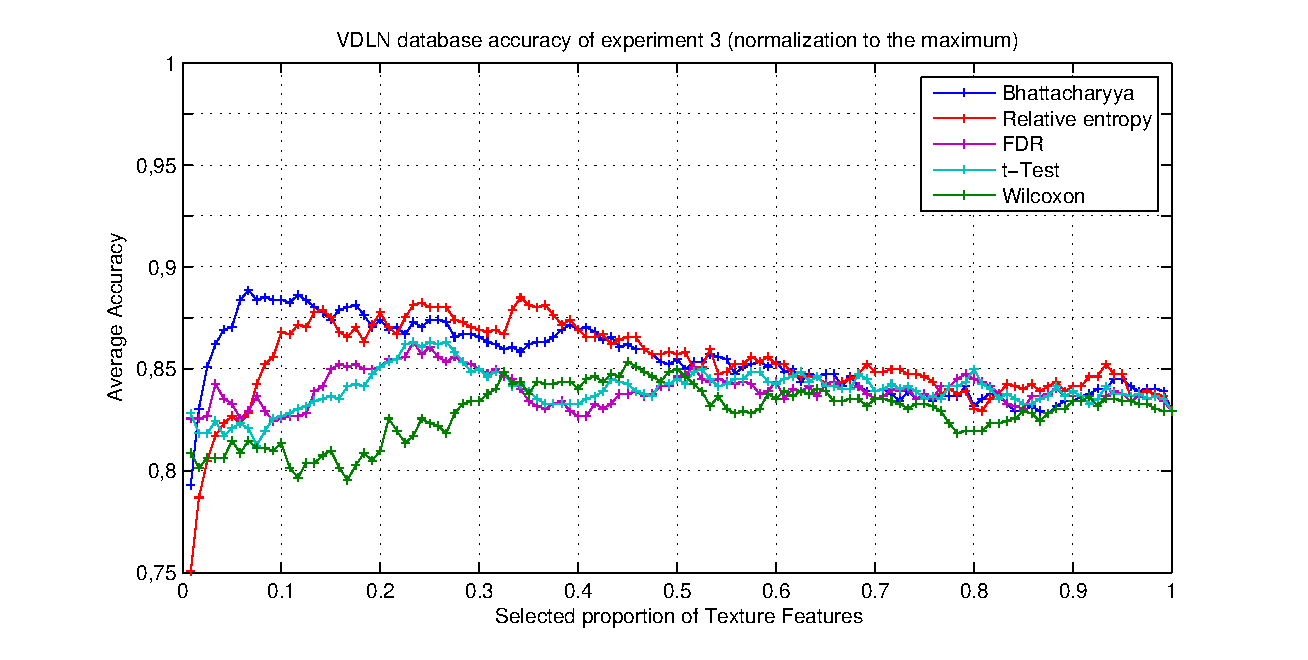
\includegraphics[width=0.5\textwidth]{Graphics/ch5/features_avAccVDLN.eps}\label{fig:experiment4-vdln}}\\
	\subfloat[VDLV-DAT]{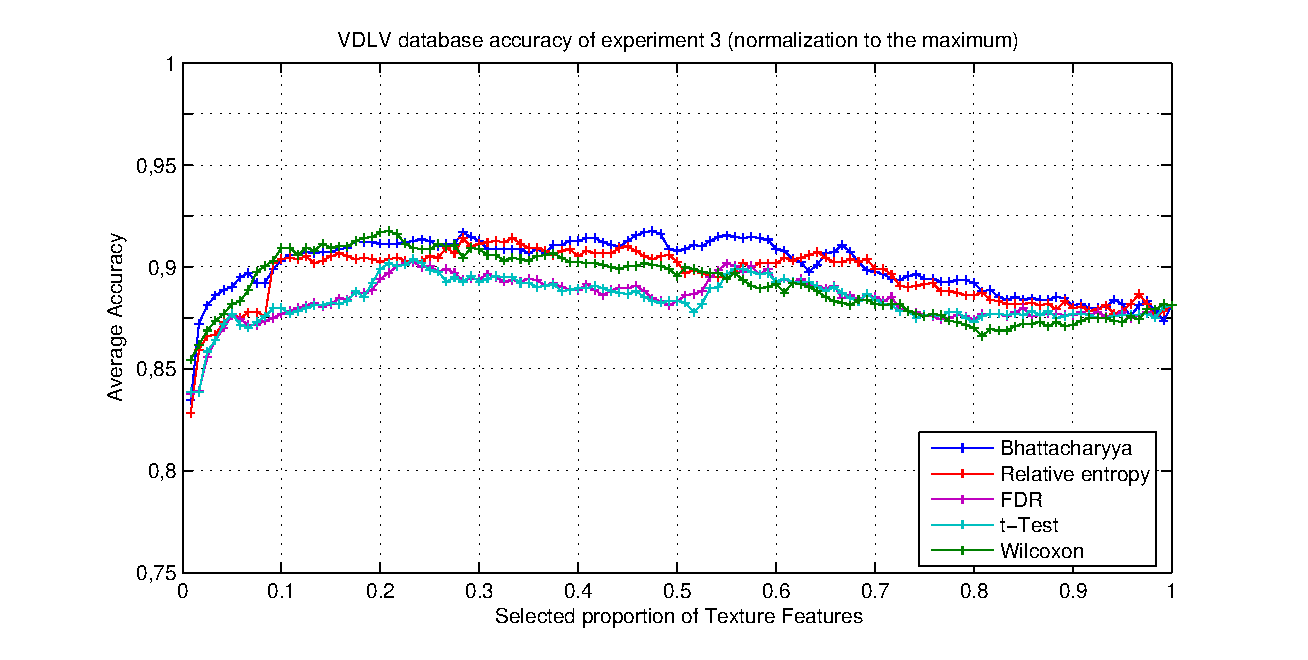
\includegraphics[width=0.5\textwidth]{Graphics/ch5/features_avAccVDLV.eps}\label{fig:experiment4-vdlv}}
	\caption[Average accuracy computed for each selection criteria over $N$ in Experiment 2.]{Average accuracy computed for each selection criteria, using all accuracy values for intensity thresholds of $0.10$ to $0.45$, compared to the proportion of selected features for the PPMI-DAT, VDLV-DAT and VDLN-DAT databases.}
	\label{fig:experiment4}
\end{figure*}

Regarding the different selection criteria, Fig.~\ref{fig:experiment4} analyses the behaviour of our system under the three proposed methods. For this purpose, we average all accuracy values for a given proportion of selected features (from 1\% to 100\% of the 1560 total texture features, previously ranked according to the selection criteria), using $I_{th}$ values ranging from 0.1 to 0.45. 

From these figures we can infer that either the $t$-test or the relative entropy criteria perform better than the \ac{MWW} U-test. Of these two, the relative entropy seems to perform the best in the PPMI-DAT and VDLN-DAT datasets, whereas when applied to the VDLV-DAT, the wilcoxon achieves similar results to the relative entropy. In these cases, the relative entropy criterion obtains its maximum average accuracy using the first 10\% of features, while wilcoxon needs more than 50\% of the features, which makes it less efficient. 

After describing the general behaviour, we can take another look at the different combinations of normalization, datasets and selection criteria. In Table~\ref{tab:exp3Res}, the peak results of these combinations are shown, including the percentage of selected features needed to achieve this value. 

\begin{table*}[htp]
	\centering
\begin{tabular}{lllccccc}
	\toprule
	                          & Norm.                  & Selection & $I_{th}$ & acc.  & sens. & spec. &  \%   \\ \midrule
	\multirow{9}{*}{PPMI-DAT} & \multirow{3}{*}{Orig.} & \textbf{entropy}   &    \textbf{30}    & \textbf{0.970} & \textbf{0.972} & \textbf{0.968} & \textbf{0.983} \\
	                          &                        & t-test    &    30    & 0.966 & 0.972 & 0.962 & 0.966 \\
	                          &                        & wilcoxon  &    30    & 0.959 & 0.954 & 0.962 & 0.858 \\ \cline{2-8}
	                          & \multirow{3}{*}{Int.}  & entropy   &    25    & 0.966 & 0.981 & 0.955 & 0.308 \\
	                          &                        & \textbf{t-test }   &    \textbf{25}    & \textbf{0.973} & \textbf{0.990 }& \textbf{0.962} &\textbf{ 0.358} \\
	                          &                        & wilcoxon  &    35    & 0.947 & 0.954 & 0.943 & 0.983 \\ \cline{2-8}
	                          & \multirow{3}{*}{Max.}  & entropy   &    25    & 0.966 & 0.981 & 0.955 & 0.308 \\
	                          &                        & \textbf{t-test}    &    \textbf{25}    &\textbf{ 0.973} & \textbf{0.990} & \textbf{0.962} & \textbf{0.358} \\
	                          &                        & wilcoxon  &    30    & 0.959 & 0.954 & 0.962 & 0.858 \\ \midrule
	\multirow{9}{*}{VDLN-DAT} & \multirow{3}{*}{Orig.} & entropy   &    30    & 0.932 & 0.933 & 0.931 & 0.175 \\
	                          &                        &\textbf{ t-test}    &    \textbf{30}    & \textbf{0.940} & \textbf{0.955} & \textbf{0.931} & \textbf{0.175} \\
	                          &                        & wilcoxon  &    15    & 0.898 & 0.955 & 0.863 & 0.433 \\ \cline{2-8}
	                          & \multirow{3}{*}{Int.}  & \textbf{entropy}   &    \textbf{25}    & \textbf{0.932} & \textbf{0.977} & \textbf{0.904} & \textbf{0.100} \\
	                          &                        & t-test    &    25    & 0.915 & 0.955 & 0.890 & 0.100 \\
	                          &                        & wilcoxon  &    25    & 0.915 & 0.911 & 0.917 & 0.966 \\ \cline{2-8}
	                          & \multirow{3}{*}{Max.}  & entropy   &    20    & 0.923 & 1.000 & 0.876 & 0.233 \\
	                          &                        & t-test    &    30    & 0.932 & 0.933 & 0.931 & 0.225 \\
	                          &                        & \textbf{wilcoxon}  &    \textbf{45}    & \textbf{0.932} & \textbf{0.933} & \textbf{0.931} & \textbf{0.033} \\ \midrule
	\multirow{9}{*}{VDLV-DAT} & \multirow{3}{*}{Orig.} & \textbf{entropy}   &    \textbf{35}    & \textbf{0.937} & \textbf{0.935} & \textbf{0.940} & \textbf{0.133 }\\
	                          &                        & t-test    &    35    & 0.932 & 0.953 & 0.910 & 0.350 \\
	                          &                        & wilcoxon  &    20    & 0.927 & 0.916 & 0.940 & 0.383 \\ \cline{2-8}
	                          & \multirow{3}{*}{Int.}  & \textbf{entropy}   &    \textbf{20}    & \textbf{0.937} & \textbf{0.935} & \textbf{0.940} & \textbf{0.983} \\
	                          &                        & t-test    &    10    & 0.932 & 0.907 & 0.960 & 0.508 \\
	                          &                        & wilcoxon  &    10    & 0.937 & 0.935 & 0.940 & 0.966 \\ \cline{2-8}
	                          & \multirow{3}{*}{Max.}  & \textbf{entropy}   &    \textbf{20}    & \textbf{0.937} & \textbf{0.953} & \textbf{0.920} & \textbf{0.608} \\
	                          &                        & t-test    &    35    & 0.932 & 0.935 & 0.930 & 0.341 \\
	                          &                        & wilcoxon  &    20    & 0.932 & 0.925 & 0.940 & 0.141 \\ \bottomrule
\end{tabular}
	\caption[Best results of the experiment 2 per database, normalization and selection criteria.]{Best results of the experiment 2 per database, normalization and selection criteria. The $I_{th}$ and percentage of selected features (of the total 1560 features computed) at which each value is obtained is also shown for comparison. }
	\label{tab:exp3Res}
\end{table*}

This table confirms that best values are obtained generally by the relative entropy criterion, with few exceptions. It also confirms that best performance is obtained when using the volume extraction method proposed in Sec.~\ref{sec:volume}, with values of $I_{th}$ between 0.25 and 0.30. As for the datasets, we see that PPMI-DAT achieves the best performance in all cases, with all selection criteria, whereas, contrary to their average performance examined in Figure~\ref{fig:averageAcc_IthNorm}, VDLN-DAT and VDLV-DAT can actually perform similarly. 

The application of intensity normalization algorithms does not imply an improvement in performance, and most systems achieve good accuracy without any normalization at all. This was pointed in other analysis, and can be checked again at this table. However, there is only one benefit that can be inferred from the table, which is a decrease in number of selected features needed to achieve best performance with the PPMI-DAT. In this case, and partially in the case of VDLN-DAT as well, similar performance is obtained using either normalized or original images, but when using the normalized data, the percentage of selected features is smaller. Nevertheless, this does not hold for the VDLV-DAT, therefore we cannot consider it a general behaviour. 

The choice of a best selection method is here a matter of trade-off between the computer performance (the number of features to estimate) and the accuracy needed. In the case of the PPMI-DAT, it is patent that using normalized images and the t-Test selection criterion achieves best performance. For VDLN-DAT is more difficult to assure that any option will perform better than others, although the t-test still performs well with the original images. Finally, with the VDLV-DAT dataset, the preferred method will be again to use the original images, since the selection of features seems more optimal, especially when using relative entropy. Anyway, all the options reveal the ability of our system in the PD detection with an relevant performance (over 90\% of accuracy in most cases). 

\section{Discussion}\label{sec:ch5discuss}
The system proposed in this chapter was published in \cite{Martinez-Murcia2013266,martinez2014parametrization}, and fundamentally defines a new pipeline for the \ac{CAD} of \ac{PD} based on texture analysis. It combines intensity normalization, a subvolume extraction algorithm, texture analysis and classification via \ac{SVC}. 

% Intensity normalization
The application of a intensity normalization procedure was proved fundamental for feature extraction methods such as \ac{VAF} \cite{Illan2012}, \ac{SVD} \cite{Segovia2012} or \ac{PLS} \cite{Rojas2012}. These methods strongly rely on the absolute intensity values found at each anatomical position. Conversely, texture analysis depends on the computation of the \ac{GLCM}, which quantifies pixel relations. When analysing the behaviour of our system in both experiments, we can infer that normalizing the images does not pose any further improvement over using the original images themselves. 

The different experiments still find improvement in using normalization, but these are very small. We find that the type of normalization depends on the database used, and no general trend could be stated. For example, VDLV-DAT has a preference for the normalization to the maximum, whereas the PPMI-DAT performs better when using integral normalization. There were even more cases where normalization decreased performance than those in which it improved the system. Therefore, we can assume that it yields no benefit at all, and therefore, our system can be intensity-independent, which we can consider an advantage. 

% Volume selection
Now, regarding the volume selection algorithm, it has proved beneficial in almost any case. This can be due to a series of reasons. Firstly, the optimum sub-volume (for an intensity threshold around $0.30 I_{max}$) has a size smaller than $40\times40\times50$. The maximum value at which we computed the \acp{GLCM} was $d=10$, which correspond to at least a 20\% of the subvolume selected with the previous value. Since the voxel size of the images in the three databases is approximately $2\times2\times2$mm, the maximum textural changes that we could analyse were computed at a distance of 20mm, approximately half the size of the striatum. This is more than enough to characterize texture in these noisy images, since lower frequency textural changes can be obviated for diagnosis, enhancing the descriptive ability of the texture features. 

Secondly, the descriptive ability of the texture features is also enhanced with the removal of the background introduced by this subvolume extraction algorithm. Within the subvolume, the texture changes only correspond to real changes represented by the dopamine distribution, and no to the contrast between the brain and the background. And thirdly, computing the texture features over a subvolume is always faster than over the whole brain, which makes our system faster. 

\begin{figure*}
	\centering
	\subfloat[Feature number (PPMI-DAT)]{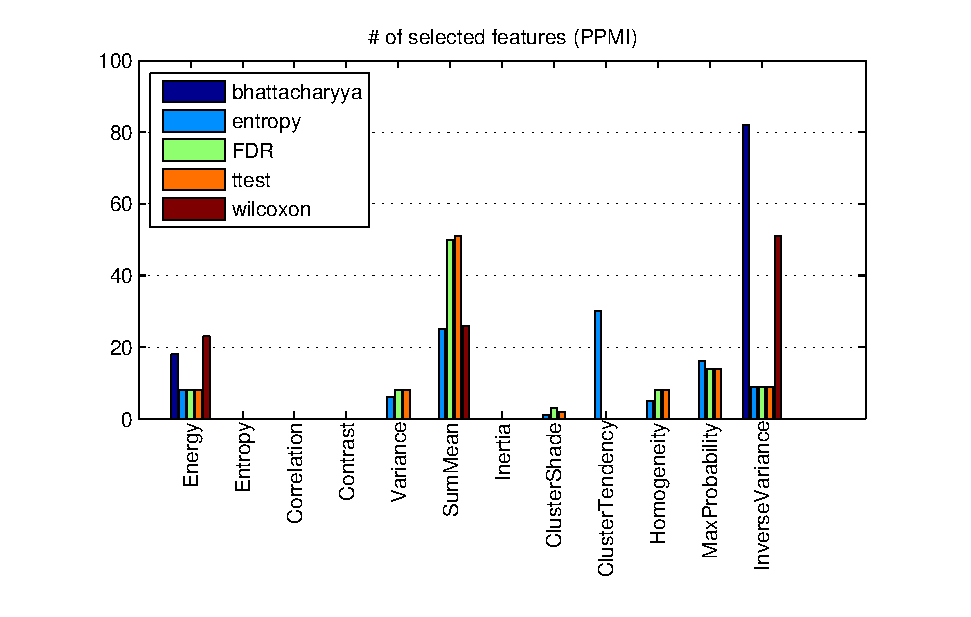
\includegraphics[width=0.5\textwidth]{Graphics/ch5/selectedFeaturesPPMI.eps}\label{fig:fnPPMI}}
	\subfloat[Feature number (VDLN-DAT)]{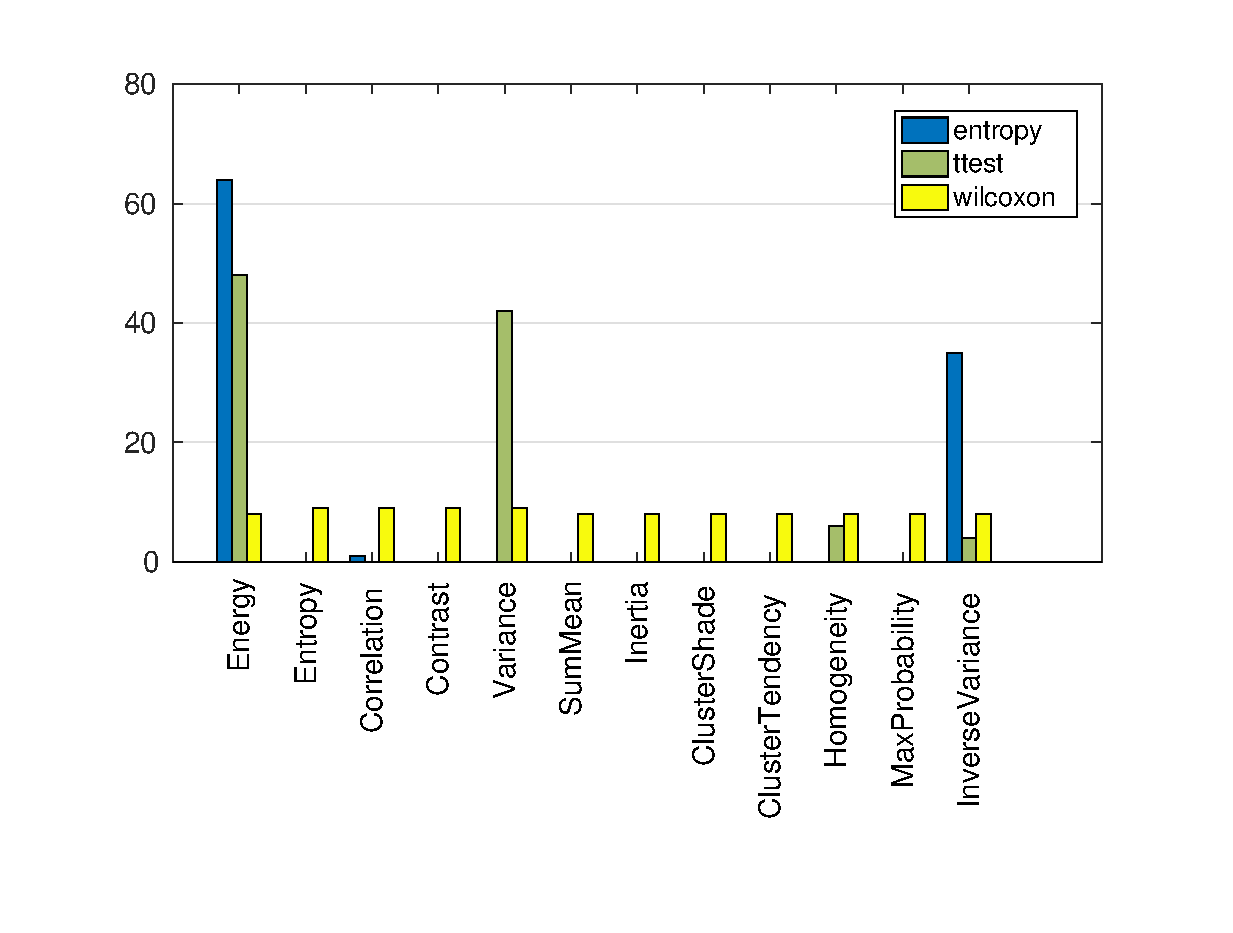
\includegraphics[width=0.5\textwidth]{Graphics/ch5/selectedFeaturesVDLN.eps}\label{fig:fnVDLN}}\\
	\subfloat[Feature number (VDLV-DAT)]{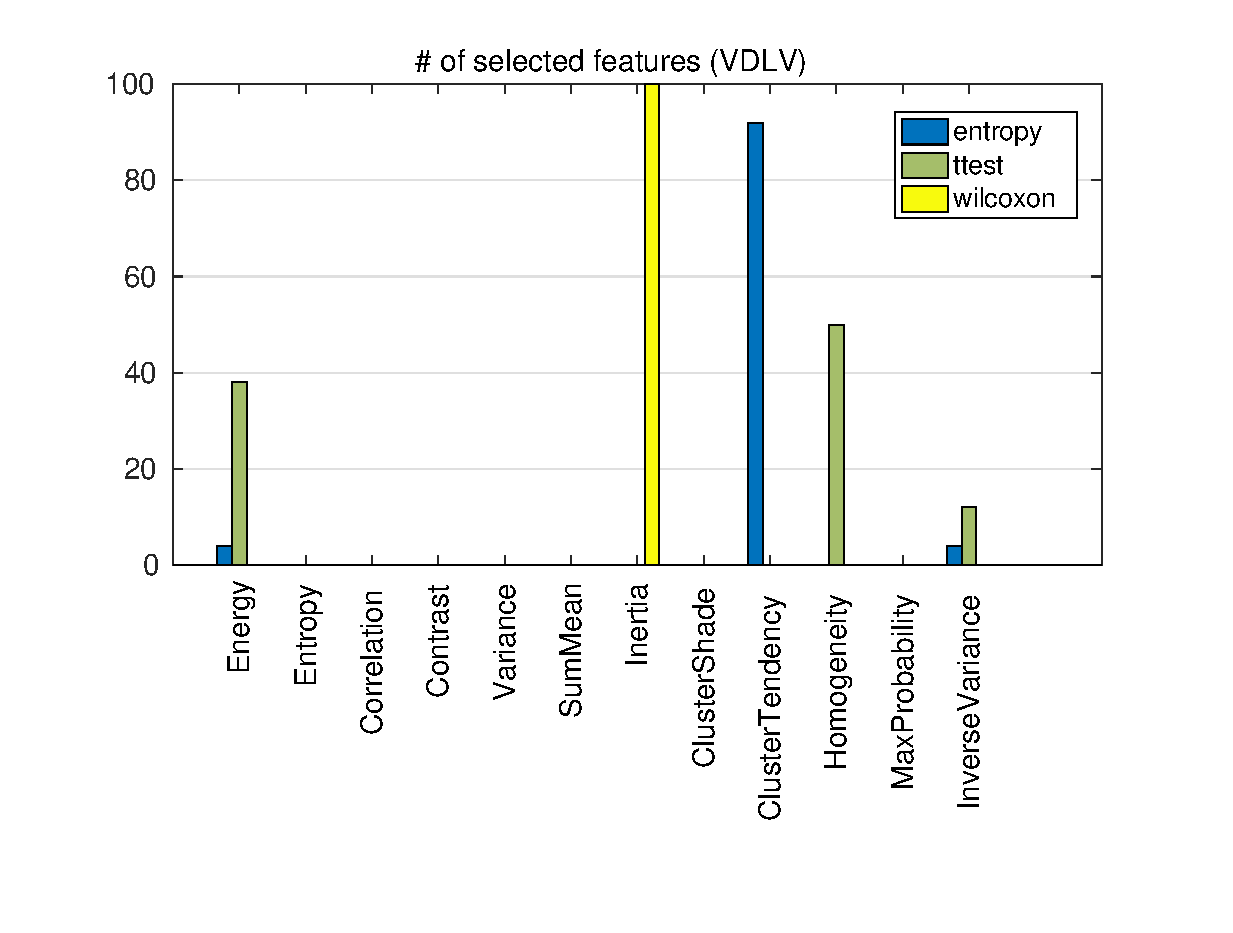
\includegraphics[width=0.5\textwidth]{Graphics/ch5/selectedFeaturesVDLV.eps}\label{fig:fnVDLV}}
	
	\caption{Distribution of the 100 first selected features by means of the different selection methods (using the $I_{th} = 0.35 I_{max}$) for PPMI-DAT, VDLN-DAT, VDLV-DAT database.} 
	\label{fig:fnumber}
\end{figure*}

% Textural features
The features that best describe the texture of DaTSCAN images are analysed in Experiment 1. In Fig.~\ref{fig:features_acc}, we saw that features such as homogeneity, Sum Mean and, overall, Cluster Tendency, achieve the best performance of our system in either the single and the cumulative approach, in all three datasets. Since Cluster tendency measures the grouping of voxels with a similar grey-level, it is obviously a good descriptor of the striatum shape, where most of the intensities of the images is concentrated. Higher values of Cluster Tendency can be associated with \ac{CTL}, whereas lower values can be related to people affected by dopaminergic deficit. 

The introduction of a feature selection algorithm using hypothesis testing improved the performance in the three datasets. Thanks to this, we can take best features according to a criterion, and use all of them regardless of what they measure. We would assume that most criteria would select fundamentally Cluster Tendency, Homogeneity and other high performance measures. In Figure~\ref{fig:fnumber} we count how many features of each type are in the 100 first ranked using each criterion and dataset. We see that the best-performing features such as cluster tendency, are not always selected, especially with the VDLN-DAT dataset, which could be responsible for its lower overall performance. It reveals that each database has internal characteristics, for example, the discarded cuts in VDLN-DAT, that are better modelled using other features, what could lead to the apparition of outliers in the computation, and a decrease in performance. However, the selection approach allow us to overcome the individual characteristics of each dataset, making the system extensible to other uses in clinical practice. 
% Whole system

Finally, we will compare our proposed system with other methods used in \ac{PD} diagnosis in the literature. We will compare with the baseline \ac{VAF} from \cite{Illan2012}, and two additional methods. These are an asymmetrical Single Value Decomposition (SVD) \cite{Segovia2012} that appplied SVD on both sides of the brain (since PD often appears only in one hemisphere), and a Empirical Mode Decomposition (EMD)  \cite{Rojas2012} using different Independent Mode Functions (IMF), particularly the IMF-3. These systems are compared with either the cumulative approach and the system of experiment 2 with different criteria in Table~\ref{tab:comparison}.

\begin{table*}[ht]
	\centering
	\begin{tabular}{l | rrr}
		\toprule
		\textbf{System}		& \textbf{Acc} 	& \textbf{Sens}	& \textbf{Spec}	\\ 
		\midrule
		SumMean &  0.951 &    0.972 &    0.936 \\ 
		Homogeneity &  0.944 &    0.946 &    0.943\\
		Cluster Shade &   0.940 &    0.936 &    0.943  \\
		Cluster Tendency &  0.951 &    0.945 &    0.956\\
		Energy &  0.936 &    0.954 &    0.924\\
		Correlation &  0.944 &    0.963 &     0.930\\
		\midrule
		Entropy       & 0.970 & 0.972 & 0.968 \\
		$t$-test       & 0.966 & 0.972 & 0.962  \\
		Wilcoxon & 0.959 & 0.954 & 0.962  \\
		\midrule
		VAF & 0.840	& 0.807	& 0.862	 \\
		VAF-IN & 0,913 & 0.890 & 0.932 \\
		SVD & 0.940 & 0.962 & 0.918 \\
		EMD-IMF3 & 0.950 & 0.951 & 0.948 \\
		\bottomrule
	\end{tabular}
	\vspace{10pt}
	\caption[Comparison between our proposed system and other \ac{PD} diagnosis systems in the literature.]{Comparison between our proposed system and other \ac{PD} diagnosis systems in the literature: a VAF system using the intensity-normalized images,  a combination of intensity normalization strategies and classifiers (VAF-IN) \cite{Illan2012}, a SVD-based approach \cite{Segovia2012} and EMD using the third independent mode function (IMF3) \cite{Rojas2012}.}
	\label{tab:comparison}
\end{table*}

In this table, we compare the values at the operation point for Experiment 1 and 2 with other methods in the literature. In Experiment 1, values for six texture features, such as Sum Mean, Homogeneity or Cluster Tendency are shown (using the single approach), and values for the three selection criteria are shown. The values of using only one texture feature match those obtained by state of the art methods like the ones proposed in \cite{Segovia2012,Rojas2012}, whereas the methodology used in Experiment 2 outperform all previously used methods. This holds for all feature selection criterion, proving the ability of the Haralick texture analysis to detect \ac{PD} patterns in DaTSCAN imaging. 
% DONE
